During the training with PCC loss the model has successfully converged already after 15 epochs however a clear overfit was encountered (see Figure \ref{fig:actin-overfit}). The reason for which is the lack of data, as for ER case there were much fewer samples than for nuclei for example (see Table \ref{table:data}). Even though one could use early-stopping approach and simply choose an earlier epoch before overfit, the better approach would be to use regularization methods described in section \ref{section:regularization}. Since the weights of the model were already regularized with a weight decay of $0.0001$ in Adadelta optimizer, the additional regularization in terms of data augmentations and Dropout layers with a dropout rate from 0.1 to 0.3 were introduced.
\begin{figure}[H]
	\begin{center}
		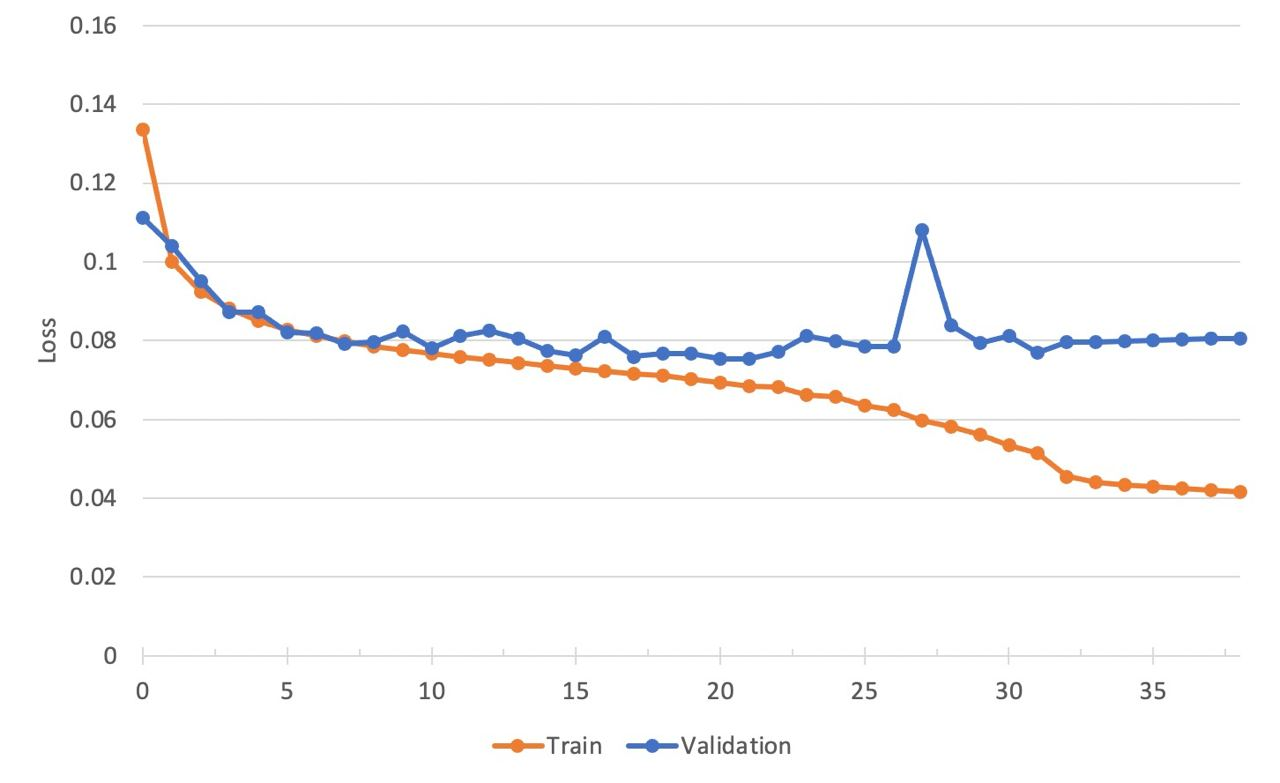
\includegraphics[width=0.5\linewidth]{bilder/actin/overfit.jpg}
		\caption{Overfit}\label{fig:actin-overfit}
	\end{center}
\end{figure}

This indeed did helps the model to escape the overfit (see Figure \ref{fig:actin-no-overfit}). Although the validation loss seem to be higher $0.072$ in comparison to $0.099$. In this case the growths were not explained by the difference between the validation sets, where the loss was measured on. PCC losses on the same validation set for both were $0.332$ and $0.315$. It might have been the case that the regularization was too strong. In order to check this the dropout layers were removed from the model and only augmentations were left (see traning and validation curves in Figure [TODO cite figure]). With the use of augmentations only PCC loss decreased to TODO and overfit TODO. Therefore it was decided to use the TODO model.
\begin{figure}[H]
	\begin{center}
		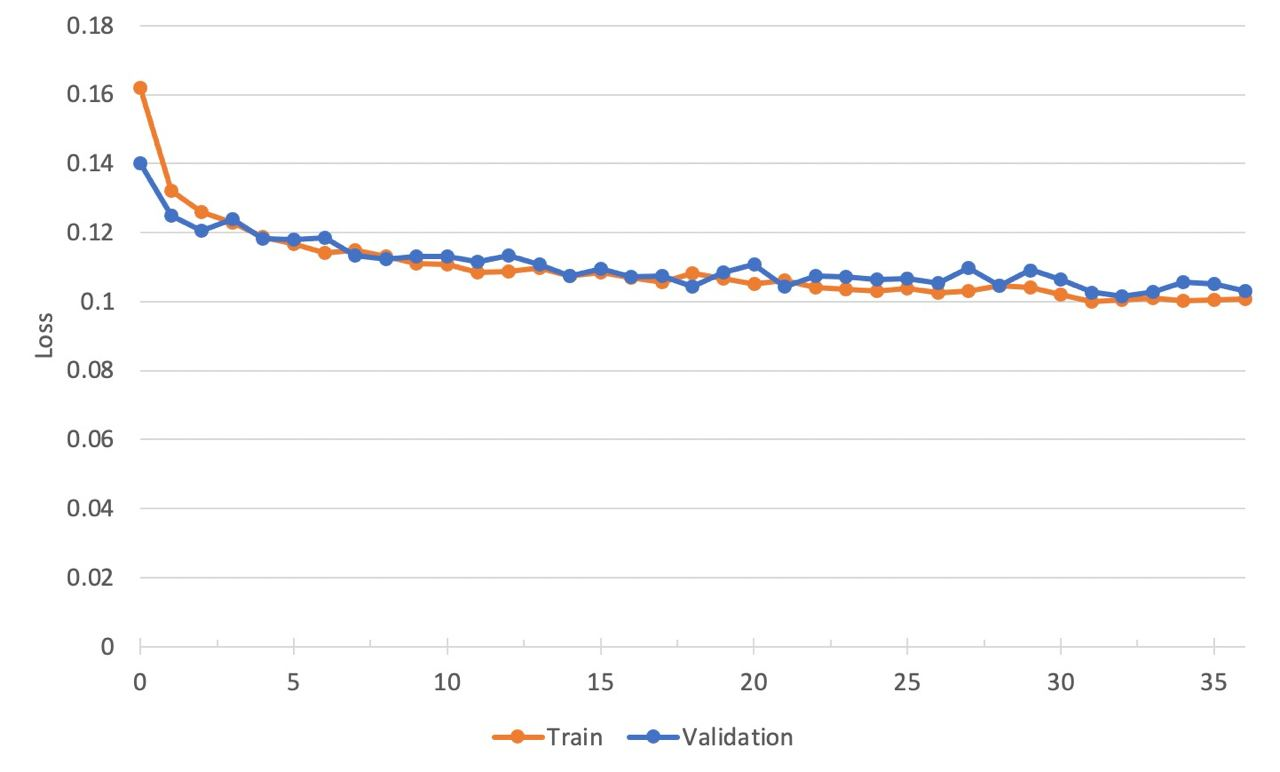
\includegraphics[width=0.5\linewidth]{bilder/actin/no-overfit.jpg}
		\caption{No overfit with augmentations}\label{fig:actin-no-overfit}
	\end{center}
\end{figure}